\chapter{Nacer, crecer, morir}\label{ch:g2:born-grow-die}

En primavera, el cerezo de la verja se cubre de \omterm{def:g1:plants-around-us:parts}{flores}; debajo, una
gata amamanta a sus gatitos recién nacidos; y el abuelo enseña una
foto de sí mismo cuando tenía tu edad --- pequeño, mellado y ya
aficionado a las cerezas. Todos los \omterm{def:g1:living-or-not:living}{seres vivos} recorren el mismo
camino: empiezan, crecen y un día se acaban. Ese camino se llama
\omterm{def:g2:born-grow-die:cycle}{ciclo de vida}.

\section{Las etapas de una vida}

\begin{definition}[Ciclo de vida]\label{def:g2:born-grow-die:cycle}
El \emph{ciclo de vida}\index{ciclo de vida} de un \omterm{def:g1:living-or-not:living}{ser vivo} es la
fila de \emph{etapas}\index{etapa} por las que pasa su vida:
\begin{enumerate}
  \item \emph{nace}\index{nacimiento} --- el comienzo;
  \item es \emph{joven}\index{joven} --- crece y cambia deprisa;
  \item es \emph{adulto}\index{adulto} --- ya ha crecido del todo;
        los adultos pueden tener crías;
  \item se hace \emph{viejo}\index{vejez} y, al final,
        \emph{muere}\index{muerte}.
\end{enumerate}
\end{definition}

\begin{example}[Tres vidas, el mismo camino]\label{ex:g2:born-grow-die:three}
Un gatito nace, juega y se convierte en una gata, que puede tener
gatitos propios, y se hace vieja. Una semilla de cerezo germina, el
árbol joven crece durante años, el árbol \omterm{def:g2:born-grow-die:cycle}{adulto} da \omterm{def:g1:plants-around-us:parts}{flores} y cerezas y,
después de muchas decenas de años, muere. Y tú: bebé, niño y un día
persona mayor. Gatito, cerezo, niño --- las mismas cuatro \omterm{def:g2:born-grow-die:cycle}{etapas}.
\end{example}

\begin{omfigure}
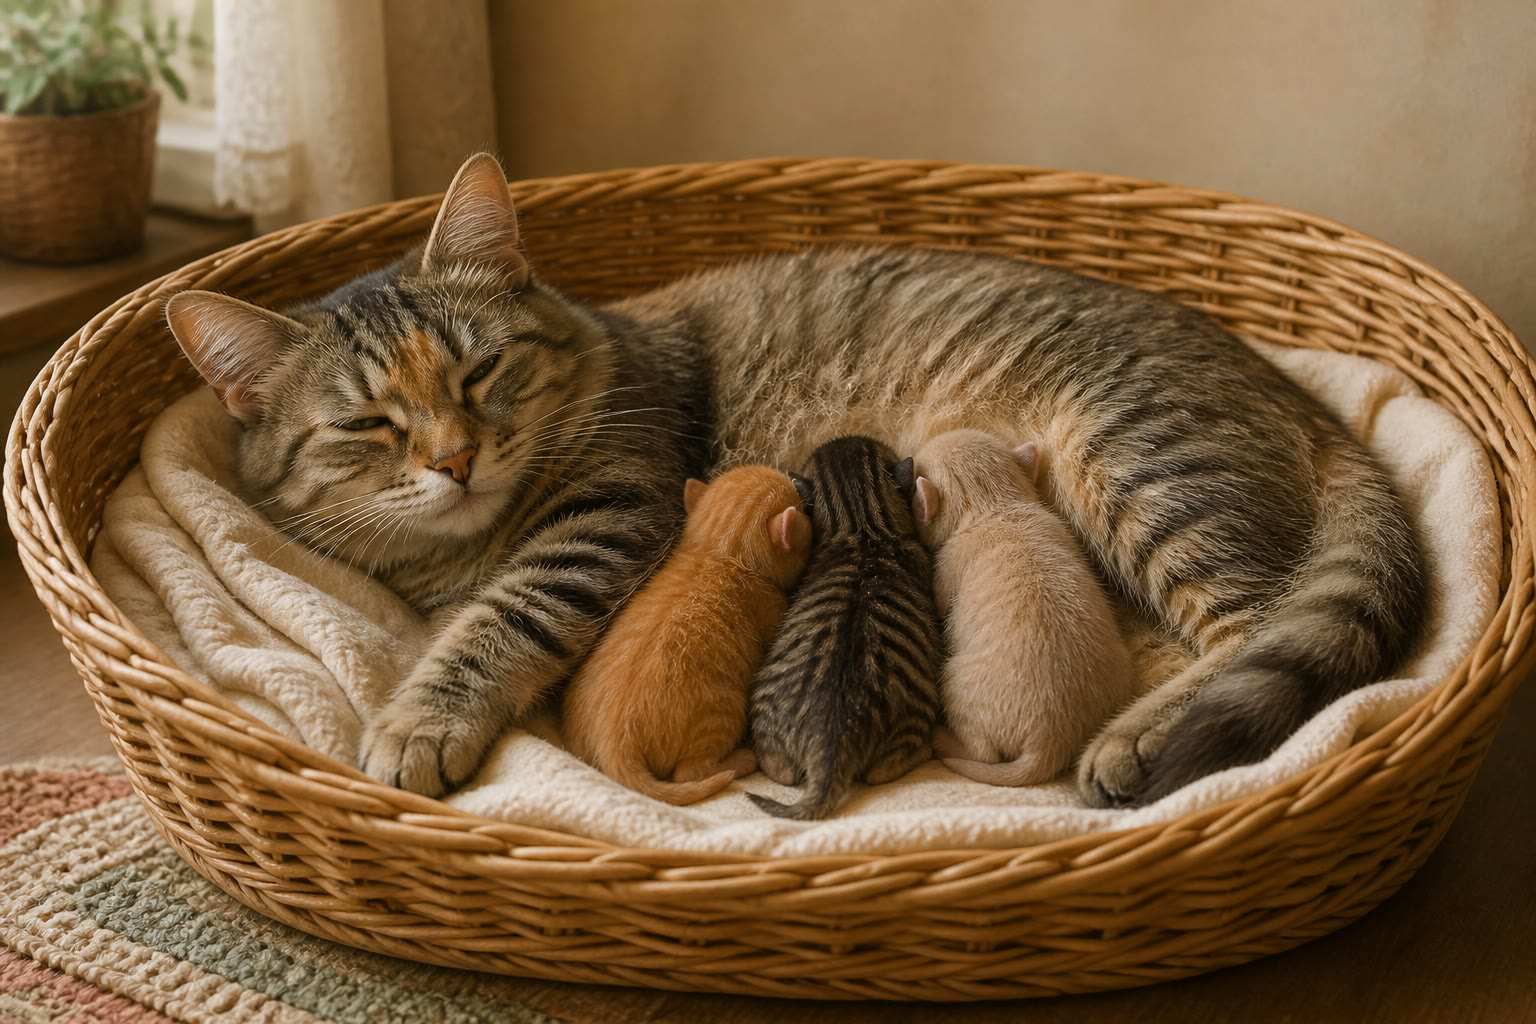
\includegraphics[width=0.62\linewidth]{images/book1/ai/g2-cycle-kittens.jpg}

{\small El comienzo de tres \omterm{def:g2:born-grow-die:cycle}{ciclos de vida} a la vez: gatitos recién
nacidos mamando de su madre.}
\end{omfigure}

\begin{omfigure}
\begin{tikzpicture}[scale=0.92]
  \foreach \x/\txt in {0/{nace},3.1/{joven},6.2/{adulto},9.3/{vejez}} {
    \draw[thick, omDef, fill=omDef!7, rounded corners=5pt]
      (\x,0) rectangle ({\x+2.4},1.2);
    \node[font=\small\bfseries, text height=1.6ex, text depth=0.4ex]
      at ({\x+1.2},0.6) {\txt};
  }
  \draw[->, thick, omMeth] (2.4,0.6) -- (3.1,0.6);
  \draw[->, thick, omMeth] (5.5,0.6) -- (6.2,0.6);
  \draw[->, thick, omMeth] (8.6,0.6) -- (9.3,0.6);
  % new generation arrow
  \draw[->, thick, omProp] (7.4,1.2) .. controls (7.4,2.3) and (1.2,2.3)
    .. (1.2,1.25);
  \node[font=\small, omProp] at (4.3,2.35) {los adultos tienen crías: empieza un ciclo nuevo};
\end{tikzpicture}

{\small Las \omterm{def:g2:born-grow-die:cycle}{etapas} de una vida --- y la flecha que vuelve a empezar el
camino con la generación siguiente.}
\end{omfigure}

\begin{remark}[Por qué se llama ciclo]\label{rem:g2:born-grow-die:wheel}
Cada vida concreta va del \omterm{def:g2:born-grow-die:cycle}{nacimiento} a la muerte, como un camino con
dos extremos. Pero antes del final los \omterm{def:g2:born-grow-die:cycle}{adultos} tienen crías, y esas
crías vuelven a empezar el camino. Vista a lo largo de muchas
generaciones, la vida gira como una rueda --- por eso decimos
\emph{ciclo} de vida.
\end{remark}

\section{Crecer y cambiar}

\begin{proposition}[Crecer es más que hacerse grande]\label{prop:g2:born-grow-die:change}
Mientras crece, un \omterm{def:g1:living-or-not:living}{ser vivo} joven también \emph{cambia}: a un bebé le
salen dientes, los pierde y le salen otros más fuertes; la pelusa
amarilla de un pollito se convierte en \omterm{def:g1:animals-around-us:covering}{plumas} de verdad; el \omterm{def:g1:plants-around-us:parts}{tallo}
verde y blando de un árbol joven se vuelve madera dura. Crecer es
hacerse más grande \emph{y} volverse distinto.
\end{proposition}
\admitted

\begin{example}[La prueba de las fotos]\label{ex:g2:born-grow-die:photo}
En las fotos antiguas del abuelo se puede seguir a una misma persona
por todas las \omterm{def:g2:born-grow-die:cycle}{etapas}: bebé, escolar, joven, padre, abuelo. La misma
persona, el cuerpo cambiando. Las fotos son maquinitas del tiempo para
ver un \omterm{def:g2:born-grow-die:cycle}{ciclo de vida}.
\end{example}

\begin{method}[Ordenar las etapas de una vida]\label{met:g2:born-grow-die:order}
Con los dibujos de la vida de un \omterm{def:g1:living-or-not:living}{ser vivo}, desordenados:
\begin{enumerate}
  \item busca el dibujo del \omterm{def:g2:born-grow-die:cycle}{nacimiento} --- huevo, semilla o recién nacido;
  \item busca el \omterm{def:g2:born-grow-die:cycle}{adulto} --- ya crecido del todo y capaz de tener crías;
  \item coloca los jóvenes en medio, de menor a mayor;
  \item repasa tu fila: ¿lleva cada dibujo al siguiente?
\end{enumerate}
\end{method}

\section{Toda vida se acaba --- y la vida sigue}

\begin{proposition}[Duración de la vida]\label{prop:g2:born-grow-die:lifespan}
Cada \omterm{def:g1:living-or-not:living}{ser vivo} vive un tiempo distinto --- su \emph{duración de la
vida}\index{duración de la vida}. Una mariposa puede vivir unas pocas
semanas; un gato, o un perro, de diez a veinte años; una persona, a
menudo más de ochenta; algunos árboles, cientos de años. Larga o
corta, toda vida tiene un final.
\end{proposition}
\admitted

\begin{example}[El manzano viejo]\label{ex:g2:born-grow-die:oldtree}
El manzano viejo y torcido del fondo del jardín da menos manzanas cada
año --- está en su \omterm{def:g2:born-grow-die:cycle}{vejez}. Pero sus manzanas tienen pepitas, y una
pepita plantada ya es un manzano joven que empieza el camino. Cuando
el árbol viejo muera, no se acabarán los manzanos: sus crías siguen.
\end{example}

\begin{remark}[Hablar de la muerte]\label{rem:g2:born-grow-die:death}
Morir forma parte de todo \omterm{def:g2:born-grow-die:cycle}{ciclo de vida}, y está bien sentirse triste
por ello --- a la gente le pasa, sobre todo con las mascotas y con las
personas a las que quiere. La \omterm{def:g1:living-or-not:living}{biología} añade un consuelo: como los
\omterm{def:g2:born-grow-die:cycle}{adultos} tienen crías antes de morir, la vida misma continúa, ciclo
tras ciclo.
\end{remark}

\section{Ejercicios}

\begin{exercise}[$\star$]\label{exo:g2:born-grow-die:1}
Nombra las cuatro \omterm{def:g2:born-grow-die:cycle}{etapas} de un \omterm{def:g2:born-grow-die:cycle}{ciclo de vida}, en orden.
\end{exercise}

\begin{exercise}[$\star$]\label{exo:g2:born-grow-die:2}
¿En qué \omterm{def:g2:born-grow-die:cycle}{etapa} puede un \omterm{def:g1:living-or-not:living}{ser vivo} tener crías propias?
\end{exercise}

\begin{exercise}[$\star$]\label{exo:g2:born-grow-die:3}
Ordena de mayor a menor edad: un escolar, un bebé, una abuela, una
madre.
\end{exercise}

\begin{exercise}[$\star$]\label{exo:g2:born-grow-die:4}
Da el \omterm{def:g2:born-grow-die:cycle}{ciclo de vida} del cerezo del \cref{ex:g2:born-grow-die:three},
\omterm{def:g2:born-grow-die:cycle}{etapa} por \omterm{def:g2:born-grow-die:cycle}{etapa}.
\end{exercise}

\begin{exercise}[$\star$]\label{exo:g2:born-grow-die:5}
Da dos ejemplos de la \cref{prop:g2:born-grow-die:change} de un \omterm{def:g1:living-or-not:living}{ser
vivo} joven que \emph{cambia} mientras crece, y no solo se hace más
grande.
\end{exercise}

\begin{exercise}[$\star$]\label{exo:g2:born-grow-die:6}
¿Quién vive normalmente más tiempo: una mariposa, un gato o un roble?
Ordena los tres por \omterm{prop:g2:born-grow-die:lifespan}{duración de la vida}.
\end{exercise}

\begin{exercise}[$\star$]\label{exo:g2:born-grow-die:7}
¿Por qué se usa la palabra \emph{ciclo}, si cada vida concreta va del
\omterm{def:g2:born-grow-die:cycle}{nacimiento} a la muerte como un camino? Usa la flecha morada de la figura.
\end{exercise}

\begin{exercise}[$\star$]\label{exo:g2:born-grow-die:8}
Pruébalo: pide a tu familia fotos de una misma persona mayor a
distintas edades y ordénalas como un \omterm{def:g2:born-grow-die:cycle}{ciclo de vida} con el
\cref{met:g2:born-grow-die:order}. ¿Qué \omterm{def:g2:born-grow-die:cycle}{etapas} enseñan las fotos? ¿Qué
\omterm{def:g2:born-grow-die:cycle}{etapa} está aún por llegar?
\end{exercise}

\begin{exercise}[$\star\star$]\label{exo:g2:born-grow-die:9}
El manzano viejo del \cref{ex:g2:born-grow-die:oldtree} morirá algún
día y, aun así, el jardín no tiene por qué quedarse sin manzanos.
Explica por qué, con la palabra \emph{generación} o con la flecha
morada de la figura.
\end{exercise}

\begin{exercise}[$\star\star$]\label{exo:g2:born-grow-die:10}
Un guijarro no muere nunca. ¿Es porque es muy resistente? Usa la idea
de vivo y no vivo del \cref{ch:g1:living-or-not} para explicarlo.
\end{exercise}
